
%% bare_conf.tex
%% V1.4b
%% 2015/08/26
%% by Michael Shell
%% See:
%% http://www.michaelshell.org/
%% for current contact information.
%%
%% This is a skeleton file demonstrating the use of IEEEtran.cls
%% (requires IEEEtran.cls version 1.8b or later) with an IEEE
%% conference paper.
%%
%% Support sites:
%% http://www.michaelshell.org/tex/ieeetran/
%% http://www.ctan.org/pkg/ieeetran
%% and
%% http://www.ieee.org/

%%*************************************************************************
%% Legal Notice:
%% This code is offered as-is without any warranty either expressed or
%% implied; without even the implied warranty of MERCHANTABILITY or
%% FITNESS FOR A PARTICULAR PURPOSE! 
%% User assumes all risk.
%% In no event shall the IEEE or any contributor to this code be liable for
%% any damages or losses, including, but not limited to, incidental,
%% consequential, or any other damages, resulting from the use or misuse
%% of any information contained here.
%%
%% All comments are the opinions of their respective authors and are not
%% necessarily endorsed by the IEEE.
%%
%% This work is distributed under the LaTeX Project Public License (LPPL)
%% ( http://www.latex-project.org/ ) version 1.3, and may be freely used,
%% distributed and modified. A copy of the LPPL, version 1.3, is included
%% in the base LaTeX documentation of all distributions of LaTeX released
%% 2003/12/01 or later.
%% Retain all contribution notices and credits.
%% ** Modified files should be clearly indicated as such, including  **
%% ** renaming them and changing author support contact information. **
%%*************************************************************************


% *** Authors should verify (and, if needed, correct) their LaTeX system  ***
% *** with the testflow diagnostic prior to trusting their LaTeX platform ***
% *** with production work. The IEEE's font choices and paper sizes can   ***
% *** trigger bugs that do not appear when using other class files.       ***                          ***
% The testflow support page is at:
% http://www.michaelshell.org/tex/testflow/



\documentclass[conference, spanish]{IEEEtran}
% Some Computer Society conferences also require the compsoc mode option,
% but others use the standard conference format.
%
% If IEEEtran.cls has not been installed into the LaTeX system files,
% manually specify the path to it like:
% \documentclass[conference]{../sty/IEEEtran}


\usepackage[spanish]{babel}
\usepackage[utf8]{inputenc}
\usepackage[T1]{fontenc}
\usepackage{caption}
\usepackage{graphicx}


\usepackage{listings}
\usepackage{color}
\usepackage{array}
\usepackage{colortbl}
\usepackage{xcolor}

\usepackage{float}
\usepackage{subfloat}
\usepackage{subfig}



% Some very useful LaTeX packages include:
% (uncomment the ones you want to load)


% *** MISC UTILITY PACKAGES ***
%
%\usepackage{ifpdf}
% Heiko Oberdiek's ifpdf.sty is very useful if you need conditional
% compilation based on whether the output is pdf or dvi.
% usage:
% \ifpdf
%   % pdf code
% \else
%   % dvi code
% \fi
% The latest version of ifpdf.sty can be obtained from:
% http://www.ctan.org/pkg/ifpdf
% Also, note that IEEEtran.cls V1.7 and later provides a builtin
% \ifCLASSINFOpdf conditional that works the same way.
% When switching from latex to pdflatex and vice-versa, the compiler may
% have to be run twice to clear warning/error messages.






% *** CITATION PACKAGES ***
%
%\usepackage{cite}
% cite.sty was written by Donald Arseneau
% V1.6 and later of IEEEtran pre-defines the format of the cite.sty package
% \cite{} output to follow that of the IEEE. Loading the cite package will
% result in citation numbers being automatically sorted and properly
% "compressed/ranged". e.g., [1], [9], [2], [7], [5], [6] without using
% cite.sty will become [1], [2], [5]--[7], [9] using cite.sty. cite.sty's
% \cite will automatically add leading space, if needed. Use cite.sty's
% noadjust option (cite.sty V3.8 and later) if you want to turn this off
% such as if a citation ever needs to be enclosed in parenthesis.
% cite.sty is already installed on most LaTeX systems. Be sure and use
% version 5.0 (2009-03-20) and later if using hyperref.sty.
% The latest version can be obtained at:
% http://www.ctan.org/pkg/cite
% The documentation is contained in the cite.sty file itself.






% *** GRAPHICS RELATED PACKAGES ***
%
\ifCLASSINFOpdf
  % \usepackage[pdftex]{graphicx}
  % declare the path(s) where your graphic files are
  % \graphicspath{{../pdf/}{../jpeg/}}
  % and their extensions so you won't have to specify these with
  % every instance of \includegraphics
  % \DeclareGraphicsExtensions{.pdf,.jpeg,.png}
\else
  % or other class option (dvipsone, dvipdf, if not using dvips). graphicx
  % will default to the driver specified in the system graphics.cfg if no
  % driver is specified.
  % \usepackage[dvips]{graphicx}
  % declare the path(s) where your graphic files are
  % \graphicspath{{../eps/}}
  % and their extensions so you won't have to specify these with
  % every instance of \includegraphics
  % \DeclareGraphicsExtensions{.eps}
\fi
% graphicx was written by David Carlisle and Sebastian Rahtz. It is
% required if you want graphics, photos, etc. graphicx.sty is already
% installed on most LaTeX systems. The latest version and documentation
% can be obtained at: 
% http://www.ctan.org/pkg/graphicx
% Another good source of documentation is "Using Imported Graphics in
% LaTeX2e" by Keith Reckdahl which can be found at:
% http://www.ctan.org/pkg/epslatex
%
% latex, and pdflatex in dvi mode, support graphics in encapsulated
% postscript (.eps) format. pdflatex in pdf mode supports graphics
% in .pdf, .jpeg, .png and .mps (metapost) formats. Users should ensure
% that all non-photo figures use a vector format (.eps, .pdf, .mps) and
% not a bitmapped formats (.jpeg, .png). The IEEE frowns on bitmapped formats
% which can result in "jaggedy"/blurry rendering of lines and letters as
% well as large increases in file sizes.
%
% You can find documentation about the pdfTeX application at:
% http://www.tug.org/applications/pdftex





% *** MATH PACKAGES ***
%
%\usepackage{amsmath}
% A popular package from the American Mathematical Society that provides
% many useful and powerful commands for dealing with mathematics.
%
% Note that the amsmath package sets \interdisplaylinepenalty to 10000
% thus preventing page breaks from occurring within multiline equations. Use:
%\interdisplaylinepenalty=2500
% after loading amsmath to restore such page breaks as IEEEtran.cls normally
% does. amsmath.sty is already installed on most LaTeX systems. The latest
% version and documentation can be obtained at:
% http://www.ctan.org/pkg/amsmath





% *** SPECIALIZED LIST PACKAGES ***
%
%\usepackage{algorithmic}
% algorithmic.sty was written by Peter Williams and Rogerio Brito.
% This package provides an algorithmic environment fo describing algorithms.
% You can use the algorithmic environment in-text or within a figure
% environment to provide for a floating algorithm. Do NOT use the algorithm
% floating environment provided by algorithm.sty (by the same authors) or
% algorithm2e.sty (by Christophe Fiorio) as the IEEE does not use dedicated
% algorithm float types and packages that provide these will not provide
% correct IEEE style captions. The latest version and documentation of
% algorithmic.sty can be obtained at:
% http://www.ctan.org/pkg/algorithms
% Also of interest may be the (relatively newer and more customizable)
% algorithmicx.sty package by Szasz Janos:
% http://www.ctan.org/pkg/algorithmicx




% *** ALIGNMENT PACKAGES ***
%
%\usepackage{array}
% Frank Mittelbach's and David Carlisle's array.sty patches and improves
% the standard LaTeX2e array and tabular environments to provide better
% appearance and additional user controls. As the default LaTeX2e table
% generation code is lacking to the point of almost being broken with
% respect to the quality of the end results, all users are strongly
% advised to use an enhanced (at the very least that provided by array.sty)
% set of table tools. array.sty is already installed on most systems. The
% latest version and documentation can be obtained at:
% http://www.ctan.org/pkg/array


% IEEEtran contains the IEEEeqnarray family of commands that can be used to
% generate multiline equations as well as matrices, tables, etc., of high
% quality.




% *** SUBFIGURE PACKAGES ***
%\ifCLASSOPTIONcompsoc
%  \usepackage[caption=false,font=normalsize,labelfont=sf,textfont=sf]{subfig}
%\else
%  \usepackage[caption=false,font=footnotesize]{subfig}
%\fi
% subfig.sty, written by Steven Douglas Cochran, is the modern replacement
% for subfigure.sty, the latter of which is no longer maintained and is
% incompatible with some LaTeX packages including fixltx2e. However,
% subfig.sty requires and automatically loads Axel Sommerfeldt's caption.sty
% which will override IEEEtran.cls' handling of captions and this will result
% in non-IEEE style figure/table captions. To prevent this problem, be sure
% and invoke subfig.sty's "caption=false" package option (available since
% subfig.sty version 1.3, 2005/06/28) as this is will preserve IEEEtran.cls
% handling of captions.
% Note that the Computer Society format requires a larger sans serif font
% than the serif footnote size font used in traditional IEEE formatting
% and thus the need to invoke different subfig.sty package options depending
% on whether compsoc mode has been enabled.
%
% The latest version and documentation of subfig.sty can be obtained at:
% http://www.ctan.org/pkg/subfig




% *** FLOAT PACKAGES ***
%
%\usepackage{fixltx2e}
% fixltx2e, the successor to the earlier fix2col.sty, was written by
% Frank Mittelbach and David Carlisle. This package corrects a few problems
% in the LaTeX2e kernel, the most notable of which is that in current
% LaTeX2e releases, the ordering of single and double column floats is not
% guaranteed to be preserved. Thus, an unpatched LaTeX2e can allow a
% single column figure to be placed prior to an earlier double column
% figure.
% Be aware that LaTeX2e kernels dated 2015 and later have fixltx2e.sty's
% corrections already built into the system in which case a warning will
% be issued if an attempt is made to load fixltx2e.sty as it is no longer
% needed.
% The latest version and documentation can be found at:
% http://www.ctan.org/pkg/fixltx2e


%\usepackage{stfloats}
% stfloats.sty was written by Sigitas Tolusis. This package gives LaTeX2e
% the ability to do double column floats at the bottom of the page as well
% as the top. (e.g., "\begin{figure*}[!b]" is not normally possible in
% LaTeX2e). It also provides a command:
%\fnbelowfloat
% to enable the placement of footnotes below bottom floats (the standard
% LaTeX2e kernel puts them above bottom floats). This is an invasive package
% which rewrites many portions of the LaTeX2e float routines. It may not work
% with other packages that modify the LaTeX2e float routines. The latest
% version and documentation can be obtained at:
% http://www.ctan.org/pkg/stfloats
% Do not use the stfloats baselinefloat ability as the IEEE does not allow
% \baselineskip to stretch. Authors submitting work to the IEEE should note
% that the IEEE rarely uses double column equations and that authors should try
% to avoid such use. Do not be tempted to use the cuted.sty or midfloat.sty
% packages (also by Sigitas Tolusis) as the IEEE does not format its papers in
% such ways.
% Do not attempt to use stfloats with fixltx2e as they are incompatible.
% Instead, use Morten Hogholm'a dblfloatfix which combines the features
% of both fixltx2e and stfloats:
%
% \usepackage{dblfloatfix}
% The latest version can be found at:
% http://www.ctan.org/pkg/dblfloatfix




% *** PDF, URL AND HYPERLINK PACKAGES ***
%
%\usepackage{url}
% url.sty was written by Donald Arseneau. It provides better support for
% handling and breaking URLs. url.sty is already installed on most LaTeX
% systems. The latest version and documentation can be obtained at:
% http://www.ctan.org/pkg/url
% Basically, \url{my_url_here}.




% *** Do not adjust lengths that control margins, column widths, etc. ***
% *** Do not use packages that alter fonts (such as pslatex).         ***
% There should be no need to do such things with IEEEtran.cls V1.6 and later.
% (Unless specifically asked to do so by the journal or conference you plan
% to submit to, of course. )


% correct bad hyphenation here
\hyphenation{op-tical net-works semi-conduc-tor}


\begin{document}
%
% paper title
% Titles are generally capitalized except for words such as a, an, and, as,
% at, but, by, for, in, nor, of, on, or, the, to and up, which are usually
% not capitalized unless they are the first or last word of the title.
% Linebreaks \\ can be used within to get better formatting as desired.
% Do not put math or special symbols in the title.
\title{VirtShell\\Framework para aprovisionamiento de soluciones virtuales}


% author names and affiliations
% use a multiple column layout for up to three different
% affiliations
\author{\IEEEauthorblockN{Carlos Alberto Llano R.}
\IEEEauthorblockA{Escuela de Ingeniería de Sistemas y Computación\\
Universidad del Valle\\
Cali, Valle del Cauca\\
Email: carlos\_llano@hotmail.com}
\and
\IEEEauthorblockN{John Alexander Sanabria}
\IEEEauthorblockA{Escuela de Ingeniería de Sistemas y Computación\\
Universidad del Valle\\
Cali, Valle del Cauca\\
Email: john.sanabria@correounivalle.edu.co}}

% conference papers do not typically use \thanks and this command
% is locked out in conference mode. If really needed, such as for
% the acknowledgment of grants, issue a \IEEEoverridecommandlockouts
% after \documentclass

% for over three affiliations, or if they all won't fit within the width
% of the page, use this alternative format:
% 
%\author{\IEEEauthorblockN{Michael Shell\IEEEauthorrefmark{1},
%Homer Simpson\IEEEauthorrefmark{2},
%James Kirk\IEEEauthorrefmark{3}, 
%Montgomery Scott\IEEEauthorrefmark{3} and
%Eldon Tyrell\IEEEauthorrefmark{4}}
%\IEEEauthorblockA{\IEEEauthorrefmark{1}School of Electrical and Computer Engineering\\
%Georgia Institute of Technology,
%Atlanta, Georgia 30332--0250\\ Email: see http://www.michaelshell.org/contact.html}
%\IEEEauthorblockA{\IEEEauthorrefmark{2}Twentieth Century Fox, Springfield, USA\\
%Email: homer@thesimpsons.com}
%\IEEEauthorblockA{\IEEEauthorrefmark{3}Starfleet Academy, San Francisco, California 96678-2391\\
%Telephone: (800) 555--1212, Fax: (888) 555--1212}
%\IEEEauthorblockA{\IEEEauthorrefmark{4}Tyrell Inc., 123 Replicant Street, Los Angeles, California 90210--4321}}




% use for special paper notices
%\IEEEspecialpapernotice{(Invited Paper)}




% make the title area
\maketitle

% As a general rule, do not put math, special symbols or citations
% in the abstract
\begin{abstract}
The abstract goes here.
\end{abstract}

% no keywords




% For peer review papers, you can put extra information on the cover
% page as needed:
% \ifCLASSOPTIONpeerreview
% \begin{center} \bfseries EDICS Category: 3-BBND \end{center}
% \fi
%
% For peerreview papers, this IEEEtran command inserts a page break and
% creates the second title. It will be ignored for other modes.
\IEEEpeerreviewmaketitle



\section{Introducción}
La aparición de ambientes de computación centrados en la nube, los cuales se caracterizan por ofrecer servicios bajo demanda, ha favorecido el desarrollo de diversas herramientas que apoyan los procesos de aprovisionamiento en demanda de servicios y ambientes de computación orientados al procesamiento de tareas de larga duración y manejo de grandes volúmenes de datos. Estos ambientes dinámicos de computación son desarrollados mayormente a través de técnicas de programación ágil las cuales se caracterizan por ofrecer rápidos resultados e integración a gran escala de componentes de software. Es así como los equipos de DevOps \footnote{DevOps consiste en traer las prácticas del desarrollo ágil a la administración de sistema y el trabajo en conjunto entre desarrolladores y administradores de sistemas. DevOps no es una descripción de cargo o el uso de herramientas, sino un método de trabajo enfocado a resultados.} se convierten en un elemento fundamental ya que potencia la estabilidad y uniformidad de los distintos ambientes de prueba y producción de modo que los procesos de integración y despliegue se hagan de forma automatizada. \\
\\
Las herramientas de aprovisionamiento automático de infraestructura son el eje central de estos equipos ya que es a través de ellas que el personal de desarrollo y operaciones son capaces de hablar un mismo lenguaje y establecer los requerimientos y necesidades a satisfacer. Sin embargo, las herramientas actuales de aprovisionamiento adolecen de servicios que faciliten la especificación de infraestructura a través de un API \footnote{ API: Application Programming Interface, conjunto de subrutinas, funciones y procedimientos que ofrece un software para ser utilizado por otro software como una capa de abstracción.} estandarizado que posibilite la orquestación del despliegue de infraestructura a través de Internet.\\
\\
En este artículo se presenta una herramienta de aprovisionamiento con orientación a servicios que permite el despliegue y orquestación de plataformas y servicios a través de un API RESTful \footnote{RESTful hace referencia a un servicio web que implementa la arquitectura REST}. Además de lo mencionado anteriormente, la artículo consta de 8 secciones.\\
\\
La segunda sección presenta el planteamiento del problema, en donde se aclara el objeto y alcance del trabajo realizado. La definición del marco teórico que permite entender la importancia de la virtualización en la actualidad, las técnicas de virtualización usadas y la sinopsis de las soluciones de aprovisionamiento mas conocidas actualmente, son presentadas en la tercera sección.\\
\\
En la cuarta sección se introduce y elabora la arquitectura planteada en VirtShell. Se describe los requisitos que se tuvieron en cuenta para elaborar la estructura del framework, las alternativas estudiadas y se reseña los módulos y sus características que conforman a VirtShell.\\
\\
Las siguientes 4 secciones se encargan de describir cada uno de los módulos diseñados, ilustrando sus funcionalidades y la forma en que interactúan de manera conjunta para administrar la infraestructura y realizar el aprovisionamiento de los recursos virtualizados. Adicionalmente se muestran ejemplos del uso del API.\\
\\
En la ultima sección se muestra la documentación del API de VirtShell. Se indican los recursos y los métodos HTTP con que cuenta cada módulo que permiten interactuar con el API.\\


\section{Problema}
En la actualidad, con la creciente adopción de modelos de computación como el \emph{Cloud Computing} \footnote{conocida también como servicios en la nube, es un paradigma que permite ofrecer servicios de computación a través de una red, que usualmente es Internet.} y el \emph{Grid Computing} \footnote{Un grid es un sistema de computación distribuido que permite coordinar computadoras de diferente hardware y software y cuyo fin es procesar una tarea que demanda una gran cantidad de recursos y poder de procesamiento.}, los ambientes computacionales se han tornado cada vez más sofisticados y complejos, requiriendo de soluciones que traten de manera integral el aprovisionamiento de diferentes servicios sobre ambientes virtuales capaces de atender la variable demanda computacional, a través del despliegue de infraestructuras elásticas de computación.\\
\\
Hoy en día, se encuentran diversas soluciones que abordan el problema de aprovisionamiento usando diferentes enfoques para el despliegue y orquestación de plataformas y servicios. Sin embargo, los enfoques actuales carecen de mecanismos de comunicación que permitan interoperar entre diferentes aplicaciones; En general, las soluciones actuales presentan dificultades para ser accedidas en una red, como internet y ejecutadas de manera remota.\\
\\
En consecuencia, para lograr la interoperabilidad con los actuales modelos de computación, este proyecto propone como objetivo principal, plantear el diseño de un framework orientado al web, cuyas partes soporten una arquitectura que permita el eficiente aprovisionamiento de software de manera automática para ambientes virtualizados. De igual modo, se propone realizar la ejemplificación del framework en un ambiente virtualizado.\\
\\
Para lograrlo será necesario evaluar diferentes estilos arquitectónicos, realizar un modelo del framework, definir la plataforma en la que se realizará la ejemplificación y definir el mecanismo de aprovisionamiento que se utilizará para aprovisionar ambientes en máquinas virtuales.\\ 



\section{Estado del arte}

La tecnología de virtualización y la computación en la nube son dos áreas de investigación muy activas. La investigación que produce estos campos es demasiada para enumerar. Cada una tiene múltiples conferencias de investigación. Por ejemplo, la ACM Symposium on Cloud Computing (SOCC) \cite{socc15} es uno de los lugares más conocidos en investigación de la computación en la nube y tecnologías de virtualización.\\
\\
La importancia de estas dos areas en la industria radica en que las nubes han transformado la forma de hacer computación. En general una empresa que use los servicios de una nube no necesita preocuparse tanto acerca de la administración de la infraestructura, las copias de seguridad, el mantenimiento, la depreciación, fiabilidad, rendimiento y tal vez de la seguridad. Estas tareas son ahora realizadas por los proveedores de la nube en otro lugar fuera de la empresa que los contrata.\\
\\
En la actualidad existen una gran oferta de nubes. Algunas de estas son públicas y están disponibles para cualquiera que esté dispuesto a pagar por el uso de los recursos, las demás son privadas para una organización. Del mismo modo, diferentes nubes ofrecen cosas diferentes. Algunas dan a sus usuarios el acceso a hardware físico, pero la mayoría permiten virtualizar sus entornos. Algunas ofrecen  las máquinas virtuales, desnudas o no, y nada más, pero otras ofrecen software que está listo para
utilizar y se pueden combinar de manera interesante, o plataformas que hacen que sea fácil para
sus usuarios desarrollar nuevos servicios \cite{tanembaum14}.\\
\\
En ese contexto, una de las principales características de la computación en la nube es la virtualización, la cual crea la ilusión de múltiples máquinas (virtuales), cada una potencialmente ejecuta un sistema operativo completamente, diferente usando el mismo hardware físico. La virtualización se puede aplicar a computadoras, sistemas operativos, dispositivos de almacenamiento de información, aplicaciones o redes. Esto permite que las empresas ejecuten mas de un sistema virtual, ademas de múltiples sistemas operativos y aplicaciones, en un único servidor, de esta manera se logra economía de escala y una mayor eficiencia.\\
\\
\subsection{Técnicas de Virtualización}
Actualmente predominan dos técnicas de virtualización. La primera técnica se denomina virtualización de hardware y consiste en que el software subyacente que ejecuta las máquinas virtuales conocido como hipervisor, crea y corre maquinas virtuales proporcionando una interfaz que es idéntica a la del servidor físico (también conocido como maquina anfitriona). El hipervisor, interactúa directamente con la CPU en el servidor físico, ofreciendo a cada uno de los servidores virtuales una total autonomía e independencia (Figura \ref{fig:hipervisor}). Incluso pueden coexistir en una misma maquina distintos servidores virtuales funcionando con distintos sistemas operativos. Esta técnica es la mas desarrollada y hay diferentes productos que cada fabricante ha ido desarrollando y adaptando, como por ejemplo Xen, KVM, VMWare y VirtualBox.\\

\begin{figure*}[!t]
\centering
\subfloat[Case I]{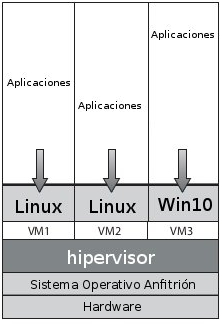
\includegraphics[width=2.5in]{../architecture/v1/diagrams/virtualmachine}%
\label{fig_first_case}}
\hfil
\subfloat[Case II]{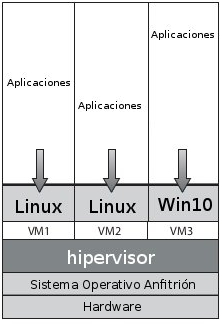
\includegraphics[width=2.5in]{../architecture/v1/diagrams/virtualmachine}%
\label{fig_second_case}}
\caption{Simulation results for the network.}
\label{fig_sim}
\end{figure*}


% \begin{figure}[h]
%   \centering
%   \caption{Máquina virtual}
%   \label{fig:hipervisor}
%   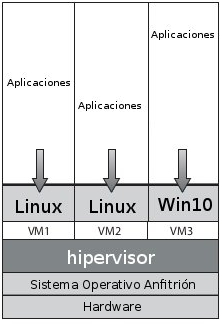
\includegraphics[width = 0.42\textwidth]{../architecture/v1/diagrams/virtualmachine}
% \end{figure}

\newpage
La segunda técnica es conocida como virtualización del sistema operativo. En esta técnica lo que se virtualiza es el sistema operativo completo el cual corre directamente sobre la maquina física. A este tipo de máquinas virtuales se les denomina contenedores, los cuales acceden por igual a todos los recursos del sistema (Figura \ref{fig:contenedores}). Esta técnica tiene una ventaja que es a su vez una desventaja: todas las máquinas virtuales usan el mismo Kernel \footnote{Kernel es un software que constituye una parte fundamental del sistema operativo, y se define como la parte que se ejecuta en modo privilegiado (conocido también como modo núcleo)}que el sistema operativo, lo que reduce los errores y multiplica el rendimiento, pero a su vez solo puede haber un mismo tipo de sistema operativo en los contenedores, no se puede combinar Windows, Linux, Etc. Este sistema también es un acercamiento a lo que seria una virtualización nativa \footnote{Tipo de virtualización en que intervienen las características del hardware. Los fabricantes preparan, sobre todo, los procesadores para que maquinas virtuales puedan trabajar con ellos más directamente.}.\\

\begin{figure}[h]
    \centering
  \caption{Contenedores}
  \label{fig:contenedores}
  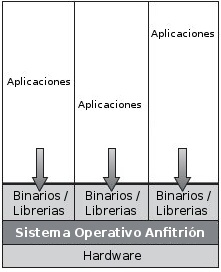
\includegraphics[width = 0.42\textwidth]{../architecture/v1/diagrams/contenedores}
\end{figure}

\newpage
De hecho, sin importar la técnica de virtualización que se use, la instalación de una maquina virtual (o de un contenedor) requiere normalmente de la generación e instalación de una imagen y a su vez de la instalación y configuración de paquetes de software. Estas tareas generalmente son realizadas por los técnicos de los proveedores de la nube. Cuando un usuario de la nube solicita un nuevo servicio o mas capacidad de computo, el administrador selecciona la imagen apropiada para clonar e instalar en los nodos de la nube. Si no existe una imagen apropiada para los requerimientos del cliente, se crea y configura una nueva que cumpla con la solicitud. Esta creación de una nueva imagen puede ser realizada modificando la imagen mas cercana de las ya existentes. En el momento de la creación optima de la imagen un administrador puede tener dificultades y preguntas como: ¿cuál es la mejor configuración?, ¿cuáles paquetes y sus dependencias deberían ser instaladas? y ¿cómo encontrar una imagen que mejor llene las expectativas?. Esto hace que la automatización y simplificación de este proceso sea una prioridad para los proveedores, ya que la depedencia entre entre paquetes de software y la dificultad de mantenimiento agrega tiempo a la creación de las máquinas virtuales. En otras palabras, uno de los principales objetivos de los proveedores de la nube es brindar mas flexibilidad y agilidad a la hora de satisfacer los requerimientos de los usuarios finales.\\
\\
\subsection{Soluciones de aprovisionamiento}
En el mercado existen muchas soluciones que permiten la interacción con diferentes ambientes de virtualización. Estas soluciones usan diferentes enfoques para realizar despliegues de software en las máquinas virtuales de manera rápida, controlada y automática. Sin embargo la mayoría de las soluciones no tienen la capacidad de manejar de manera simultanea las dos técnicas de virtualización antes mencionadas, algunas se centran solo en manejar máquinas virtuales y otras pocas solo hacen aprovisionamiento sobre contenedores.\\
\\
Así mismo, hay soluciones de aprovisionamiento que han incorporado su propio lenguaje buscando mayor flexibilidad y fácil configuración de las tareas. Sin embargo, esto implica incorporar una curva de aprendizaje bastante alta, lo que se traduce en un gran esfuerzo inicial para contar con toda la infraestructura automatizada. En ese mismo orden de ideas, existen a su vez, soluciones cuya curva de aprendizaje es mucho menor lo que las hace mas atractivas para muchos ingenieros de Tecnologías de la Información (TI).\\
\\
Adicionalmente, así como se encuentran soluciones o herramientas de aprovisionamiento de desarrollo propietario que cobran por sus funcionalidades mas importantes o por el numero de máquinas que pueden aprovisionar, existen herramientas de código abierto o de uso libre que permiten trabajar con un número considerable de máquinas virtuales. Al revisar alrededor de 40 diferentes herramientas de aprovisionamiento se logro identificar dos características que no se encuentran en las soluciones actuales. La primera trata de la ausencia de una interfaz o API web para realizar aprovisionamiento remoto y la segunda se refiere a que las herramientas se limitan a aprovisionar las máquinas virtuales sin ofrecer mecanismos de administración y monitoreo de la red aprovisionada o de los anfitriones que albergan los recursos virtuales.\\
\\
A continuación se describirán algunas de las herramientas mas conocidas actualmente son descritas a continuación:

\begin{description}
\item [Fabric]
 es una herramienta de automatización que usa SSH \footnote{SSH (Secure SHell, en español: intérprete de órdenes seguro) es el nombre de un protocolo y del programa que lo implementa, y sirve para acceder a máquinas remotas a través de una red} para hacer despliegues de aplicaciones y administración de tareas. Fabric es una librería gratuita hecha en python y su forma de interactuar es por medio de linea de comandos. Por otra parte permite cargar y descargar archivos que pueden ser ejecutados por su conjunto de funciones \cite{fabfile16}.

\item [Chef]
es una de las herramientas más conocidas de automatización de infraestructura de nube, esta escrita en Ruby y Erlang. Utiliza un lenguaje de dominio especifico, expresado también en Ruby para la escritura y configuracion de los recursos que deben ser creados, a esto se le denomina "recetas". Estas recetas contienen los recursos que deben ser creados. Chef se puede integrar con plataformas basadas en la nube, como Rackspace, Internap, Amazon EC2, Cloud Platform Google, OpenStack, SoftLayer y Microsoft Azure. Adicionalmente puede aprovisionar sobre contenedores si se instala la librería indicada. \\
\\
Chef contiene soluciones para sistemas de pequeña y gran escala \cite{Chef15}.Es uno de los cuatro principales sistemas de gestión de configuración en Linux, junto con Cfengine, Bcfg2 y Puppet. La version gratuita puede ser utilizada, pero no cuenta con todo el conjunto de caracteristicas, administracion y soporte brindados por la herramienta. Estos se pueden obtener pagando una licencia de uso.


\item [Puppet]
es una herramienta diseñada para administrar la configuración de sistemas similares a Unix y a Microsoft Windows de forma declarativa. El usuario describe los recursos del sistema y sus estados utilizando el lenguaje declarativo que proporciona Puppet. Esta información es almacenada en archivos denominados manifiestos Puppet. Puppet descubre la información del sistema a través de una utilidad llamada Facter, y compila los manifiestos en un catalogo especifico del sistema que contiene los recursos y las dependencias de dichos recursos, estos catálogos son ejecutados en los sistemas de destino \cite{Pupet15}. Puppet es de uso gratuito para redes muy pequeñas de hasta solo 10 nodos.

\item [Juju]
 es una herramienta de configuración y administración de servicios en nubes publicas. Permite crear ambientes completos con unos pocos comandos, cuenta con cientos de servicios pre-configurados y disponibles en la tienda de juju. Se puede usar a través de una interfaz gráfica o de linea de comandos. Juju permite re-crear un ambiente de producción en portátiles usando contenedores enfocado a pruebas. El uso de juju es gratuito pero se debe pagar por el uso de la nube publica \cite{juju16}.

\item [CFEngine]
es un sistema basado en el lenguaje escrito por Mark Burgess, diseñado específicamente para probar y configurar software. CFEngine es como un lenguaje de muy alto nivel. Su objetivo es crear un único archivo o conjunto de archivos que describen la configuración de cada máquina de la red. CFEngine se ejecuta en cada host, y analiza cada archivo (o archivos), que especifica una política para la configuración del sistema. La configuración de la máquina es verificada contra el modelo y, si es necesario, cualquier desviación de la configuración es corregida. \cite{cfengine15}\\
\\
CFEngine cuenta con una versión gratuita y la versión empresarial que cuenta con interfaz gráfica, soporte y reportes.

\item [Ansible]
es una herramienta de código libre desarrollada en python y comercialmente ofrecida por AnsibleWorks los cuales la definen como un motor de orquestación muy simple que automatiza las tareas de despliegue. Ansible no usa agentes, solo necesita tener instalado Python en las máquinas hosts y las tareas las realiza por medio de ssh. Ansible puede trabajar mediante un solo archivo de configuración que contendría todo o por medio de varios archivos organizados en una estructura de directorios \cite{ans16}. 

\item [Bcfg2]
esta escrito en Python y permite gestionar la configuración de un gran numero de ordenadores mediante un modelo de configuración central. Bcfg2 funciona con un modelo simple de configuración del sistema, modelando elementos intuitivos como paquetes, servicios y archivos de configuración (así como las dependencias entre ellos). Este modelo de configuración del sistema se utiliza para la verificación  y validación de las máquinas, permitiendo una auditoria robusta de los sistemas desplegados. La especificación de la configuración de Bcfg2 está escrita utilizando un modelo XML declarativo. Toda la especificacion puede ser validada utilizando los validadores de esquema XML ampliamente disponibles. Bcfg2 no tiene soporte para contenedores. Es gratuito y cuenta con una lista limitada de plataformas en las cuales trabaja bien.\cite{bdfg215}

\item [Cobbler]
 es una plataforma que busca el rápido despliegue de servidores y en general computadores en una infra-estructura de red por medio de linea de comandos, se basa en el modelo de scripts y cuenta con una completa base de simples comandos, que permite hacer despliegues de manera rápida y con poca intervención humana. Cobbler es capaz de instalar máquinas físicas y máquinas virtuales. Cobbler, es una pequeña y ligera aplicacion, que es extremadamente facil de usar para pequeños o muy grandes despliegues. Es de uso gratuito y no cuenta con soporte para contenedores. \cite{Cobbler15}

\item [SmartFrog]
 es un framework para servicios de configuración, descripción, despliegue y administración del ciclo de vida de máquinas virtuales. Consiste de un lenguaje declarativo, un motor que corre en los nodos remotos y ejecuta plantillas escritas en el lenguaje de SmartFrog y un modelo de componentes. El lenguaje soporta encapsulación (que es similar a las clases de python), herencia y composición que permite personalizar y combinar configuraciones. SmartFrog, permite enlaces estáticos y dinámicos entre componentes, que ayudan a soportar diferentes formas de conexión en tiempo de despliegue.\\
\\
El modelo de componentes, administra el ciclo de vida a través de cinco estados: instalado, iniciado, terminado y fallido. Esto permite al motor del SmartFrog detectar fallas y reiniciar automáticamente re-despliegues de los componentes \cite{Smart09}.\\
\\
SmartFrog es desarrollado y mantenido por un equipo de investigación en los laboratorios de Hewlett-Packard en Bristol, Inglaterra, así como por el laboratorio Europeo de Hewlett-Packard y por contribuciones de otros usuarios de SmartFrog y desarrolladores externos a HP. Se utiliza en la investigación de HP, específicamente en la automatización de la infraestructura y automatización de servicios, ademas de ser solo utilizado en determinados productos de HP.

\item [Amazon EC2]
es un API propietario de Amazon que maneja un enfoque manual, el cual permite desplegar imágenes de máquinas virtuales conocidas como AMI (Amazon Machine Images) \cite{Amazon16}, que son las imágenes que se utilizan en Amazon para arrancar instancias virtuales. El concepto de las AMIs \footnote{La AMI de Amazon es una imagen mantenida y compatible que ofrece Amazon Web Services para su uso en Amazon Elastic Compute Cloud (Amazon EC2).} es similar a las máquinas virtuales de otros sistemas. Básicamente estan compuestas de una serie de ficheros de datos que conforman la imagen y luego un xml que especifica ciertos valores necesarios para que sea una imagen valida para Amazon. 

\item [Docker composer]
permite describir un conjunto de contenedores que se relacionan entre ellos. Docker composer define una aplicación multicontenedor en un archivo con las mismas propiedades que se indicarían en un archivo individual de docker. Docker composer usa archivos en formato yaml para describir las características de los servicios en cada contenedor \cite{doccom16}. Es completamente gratuito. 

\item [Vagrant]
 es una herramienta de linea de comando que permite la creación y configuración de entornos de desarrollo virtualizados. Originalmente se desarrolló para VirtualBox y sistemas de configuración tales como Chef, Salt y Puppet. Sin embargo desde la versión 1.1 Vagrant es capaz de trabajar con múltiples proveedores, como VMware, Amazon EC2, LXC y DigitalOcean \cite{Vag15}.\\
\\
Vagrant ofrece múltiples opciones para realizar aprovisionamientos, desde scritps en shell hasta complejos sistemas de configuración.

\item [SaltStack]
 es un sistema de manejo de configuración cuyo objetivo es garantizar que un servicio este corriendo o que una aplicación haya sido instalada o desplegada. Salt está construido en Python y al igual que Chef, CFEngine y Puppet utiliza un esquema de cliente (salt minions) - servidor (salt master), cuyo método de conexión con los minions se realiza a través de un broker messages \footnote{es un programa intermediario que traduce los mensajes de un sistema desde un lenguaje a otro, a través de un medio de telecomunicaciones.} llamado ZeroMQ (0MQ), que no solo garantiza una conexión segura sino que la hace confiable y rápida. Salt tiene una versión gratuita llamada Salt Open sin embargo para obtener todos los beneficios se debe pagar la versión empresarial. Salt cuenta con soporte para contenedores. \cite{Salt15}

\end{description}


% An example of a floating figure using the graphicx package.
% Note that \label must occur AFTER (or within) \caption.
% For figures, \caption should occur after the \includegraphics.
% Note that IEEEtran v1.7 and later has special internal code that
% is designed to preserve the operation of \label within \caption
% even when the captionsoff option is in effect. However, because
% of issues like this, it may be the safest practice to put all your
% \label just after \caption rather than within \caption{}.
%
% Reminder: the "draftcls" or "draftclsnofoot", not "draft", class
% option should be used if it is desired that the figures are to be
% displayed while in draft mode.
%
%\begin{figure}[!t]
%\centering
%\includegraphics[width=2.5in]{myfigure}
% where an .eps filename suffix will be assumed under latex, 
% and a .pdf suffix will be assumed for pdflatex; or what has been declared
% via \DeclareGraphicsExtensions.
%\caption{Simulation results for the network.}
%\label{fig_sim}
%\end{figure}

% Note that the IEEE typically puts floats only at the top, even when this
% results in a large percentage of a column being occupied by floats.


% An example of a double column floating figure using two subfigures.
% (The subfig.sty package must be loaded for this to work.)
% The subfigure \label commands are set within each subfloat command,
% and the \label for the overall figure must come after \caption.
% \hfil is used as a separator to get equal spacing.
% Watch out that the combined width of all the subfigures on a 
% line do not exceed the text width or a line break will occur.
%
%\begin{figure*}[!t]
%\centering
%\subfloat[Case I]{\includegraphics[width=2.5in]{box}%
%\label{fig_first_case}}
%\hfil
%\subfloat[Case II]{\includegraphics[width=2.5in]{box}%
%\label{fig_second_case}}
%\caption{Simulation results for the network.}
%\label{fig_sim}
%\end{figure*}
%
% Note that often IEEE papers with subfigures do not employ subfigure
% captions (using the optional argument to \subfloat[]), but instead will
% reference/describe all of them (a), (b), etc., within the main caption.
% Be aware that for subfig.sty to generate the (a), (b), etc., subfigure
% labels, the optional argument to \subfloat must be present. If a
% subcaption is not desired, just leave its contents blank,
% e.g., \subfloat[].


% An example of a floating table. Note that, for IEEE style tables, the
% \caption command should come BEFORE the table and, given that table
% captions serve much like titles, are usually capitalized except for words
% such as a, an, and, as, at, but, by, for, in, nor, of, on, or, the, to
% and up, which are usually not capitalized unless they are the first or
% last word of the caption. Table text will default to \footnotesize as
% the IEEE normally uses this smaller font for tables.
% The \label must come after \caption as always.
%
%\begin{table}[!t]
%% increase table row spacing, adjust to taste
%\renewcommand{\arraystretch}{1.3}
% if using array.sty, it might be a good idea to tweak the value of
% \extrarowheight as needed to properly center the text within the cells
%\caption{An Example of a Table}
%\label{table_example}
%\centering
%% Some packages, such as MDW tools, offer better commands for making tables
%% than the plain LaTeX2e tabular which is used here.
%\begin{tabular}{|c||c|}
%\hline
%One & Two\\
%\hline
%Three & Four\\
%\hline
%\end{tabular}
%\end{table}


% Note that the IEEE does not put floats in the very first column
% - or typically anywhere on the first page for that matter. Also,
% in-text middle ("here") positioning is typically not used, but it
% is allowed and encouraged for Computer Society conferences (but
% not Computer Society journals). Most IEEE journals/conferences use
% top floats exclusively. 
% Note that, LaTeX2e, unlike IEEE journals/conferences, places
% footnotes above bottom floats. This can be corrected via the
% \fnbelowfloat command of the stfloats package.




\section{Conclusion}
The conclusion goes here.




% conference papers do not normally have an appendix


% use section* for acknowledgment
\section*{Acknowledgment}


The authors would like to thank...





% trigger a \newpage just before the given reference
% number - used to balance the columns on the last page
% adjust value as needed - may need to be readjusted if
% the document is modified later
%\IEEEtriggeratref{8}
% The "triggered" command can be changed if desired:
%\IEEEtriggercmd{\enlargethispage{-5in}}

% references section

% can use a bibliography generated by BibTeX as a .bbl file
% BibTeX documentation can be easily obtained at:
% http://mirror.ctan.org/biblio/bibtex/contrib/doc/
% The IEEEtran BibTeX style support page is at:
% http://www.michaelshell.org/tex/ieeetran/bibtex/
%\bibliographystyle{IEEEtran}
% argument is your BibTeX string definitions and bibliography database(s)
%\bibliography{IEEEabrv,../bib/paper}
%
% <OR> manually copy in the resultant .bbl file
% set second argument of \begin to the number of references
% (used to reserve space for the reference number labels box)
\begin{thebibliography}{1}

\bibitem{IEEEhowto:kopka}
H.~Kopka and P.~W. Daly, \emph{A Guide to \LaTeX}, 3rd~ed.\hskip 1em plus
  0.5em minus 0.4em\relax Harlow, England: Addison-Wesley, 1999.



\bibitem{socc15} ACM Symposium on Cloud Computing 2015, http://acmsocc.github.io/2015, 2015.

\bibitem{tanembaum14} Andrew S. Tanembaum, Modern Operating Systems 4th Edition, 2014.

\bibitem{fabfile16}Fabric, http://www.fabfile.org/, 2016.

\bibitem{juju16}Ubuntu Juju, http://www.ubuntu.com/cloud/juju, 2016.

\bibitem{doccom16}Docker Composer, https://docs.docker.com/compose, 2016.

\bibitem{Smart09}SmartFrog, http://smartfrog.org/display/sf/SmartFrog+Home, 2009.

\bibitem{ans16}Ansible, https://www.ansible.com, 2016.

\bibitem{Amazon16}Amazon EC2, https://aws.amazon.com/ec2, 2016.

\bibitem{Chef15}Chef, https://docs.chef.io, 2015.

\bibitem{Pupet15}Puppet, http://projects.puppetlabs.com/projects/puppet, 2015.

\bibitem{cfengine15}Cfengine, https://www.gnu.org/software/cfengine, 2001.

\bibitem{bdfg215}Bdfg2, http://bcfg2.org, 2015.

\bibitem{Cobbler15}Cobbler, https://cobbler.github.io, 2016.

\bibitem{Vag15}Vagrant, https://www.vagrantup.com, 2016.

\bibitem{Salt15}SaltStack, http://saltstack.com/community, 2016.

\bibitem{fielding00} Architectural Styles and
the Design of Network-based Software Architectures, https://www.ics.uci.edu/~fielding/pubs/dissertation/top.htm, 2000.

\bibitem{fowler04} Inversion of Control Containers and the Dependency Injection pattern, http://martinfowler.com/articles/injection.html, 2004.

\bibitem{rfc2104}HMAC: Keyed-Hashing for Message Authentication, https://www.ietf.org/rfc/rfc2104.txt, 1997.

\bibitem{lxc16}Linux Containers, https://linuxcontainers.org, 2016..

\bibitem{lxcubuntu16}LXC Templates Documentation, https://help.ubuntu.com/lts/serverguide/lxc.html, 2016.

\bibitem{docker16}Docker, https://docker.com, 2016.

\bibitem{Xinyang09} REST - An Alternative to RPC for Web Services Architecture, http://web.uvic.ca/\~erikj/seng422/resources/rest\_paper.pdf, 2009.



\end{thebibliography}




% that's all folks
\end{document}


